\subsection{Inicio de sesión}

\begin{figure}[H]
\centerline{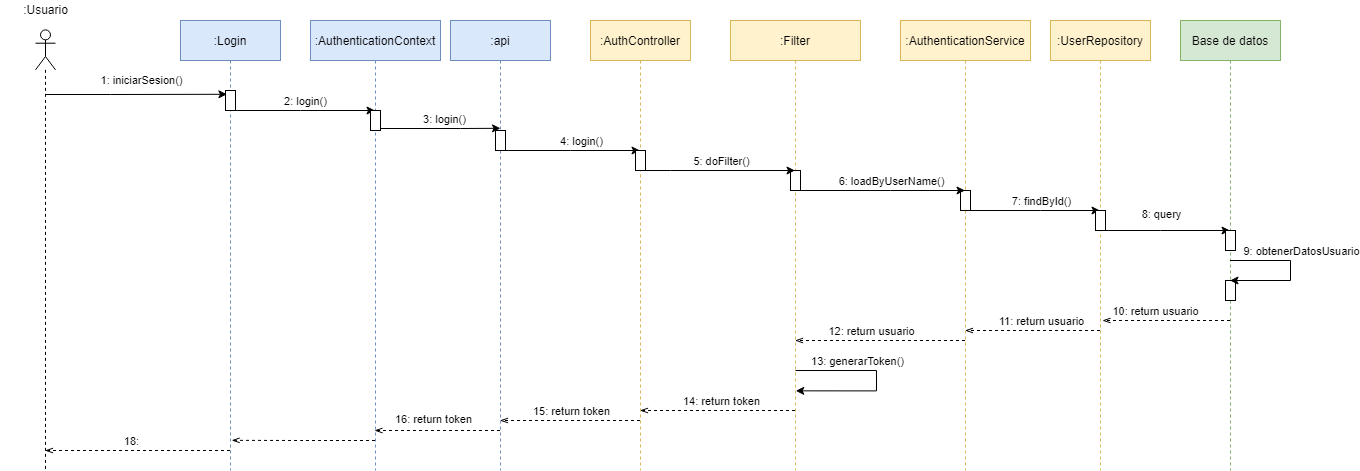
\includegraphics[width=13cm]{figuras/diseño/IniciarSesion.png}}
\caption{Diagrama de secuencia del inicio de sesión.}
\label{enlaceDInicioSesionCuerpo}
\end{figure}

El inicio de sesión es una de las funcionalidades más importantes del sistema. Si un usuario no tiene iniciada la sesión, no se permitirá en ningún caso el uso de la aplicación. El inicio de sesión se realizará mediante el correo electrónico y la contraseña de un usuario, y el diagrama de secuencia correspondiente se puede observar en la \hyperref[enlaceDInicioSesionCuerpo]{Figura 3.10}. Se describe a continuación el proceso:

\begin{enumerate}
    \item El usuario, tras introducir su correo y contraseña, pincha en iniciar sesión en la página de {\bf Login}.
    \item Se llama a la función {\it login()} de {\bf AuthenticationContext}, que es donde se gestionan todos los datos de inicio de sesión de un usuario en el cliente.
    \item Se hace un llamamiento al método {\it login()} de la carpeta {\bf api}, para que se localice el método en el servidor.
    \item {\bf AuthController} detecta que se desea iniciar sesión porque recibe una solicitud HTTP de tipo POST a su método {\it login()}.
    \item Se hacen pasar los datos del usuario por los filtros de la carpeta {\bf Filter} para comprobar que los datos son correctos.
    \item Para que los filtros puedan comprobar que los datos son correctos, deben obtener los datos del usuario, por ello, hacen un llamamiento al método {\it loadByUserName()} de {\bf AuthenticationService}.
    \item Se busca el usuario en el repositorio {\bf UserRepository} mediante el método {\it findById()}.
    \item El repositorio hace una {\it query} a la base de datos de MongoDB invocando al método de obtención de usuarios.
    \item La base de datos busca el usuario correspondiente en la base de datos.
    \item En caso de encontrar el usuario, este se devuelve a los filtros.
    \item Si los datos de inicio de sesión son correctos, se genera un token JWT de inicio de sesión.
    \item Este token se devuelve hasta {\bf AuthenticationContext}, para que se encargue de almacenar los datos en el almacenamiento local del cliente.
    \item Por último, se indica al usuario que el inicio de sesión fue realizado.
\end{enumerate}